% The key aspects to preserve are the \chapter, the \bibliography, and the \subappendices commands. For the rest, there should be full flexibility
\chapter{Title paper 1}

%% Text of abstract
\begin{abstract}
\noindent   \lipsum[9-9]
\end{abstract}

\noindent   \textit{Keywords:}      \newline
            \textit{JEL Codes:}



\pagebreak
\setlength\epigraphwidth{10cm}
\setlength\epigraphrule{0pt}
\epigraph{      \flushright{\textit{Quote for Paper 1}} }   

% main text
\section{Introduction}

\lipsum[8-8] As in table (\ref{paper1_table_frequency}), ...

\begin{center}
    \vspace{0.3cm}
    \textit{[Table \ref{paper1_table_frequency}]}
    \vspace{0.3cm}
\end{center}

\section{The analysis}

\begin{figure}[hbt!]
    \centering
    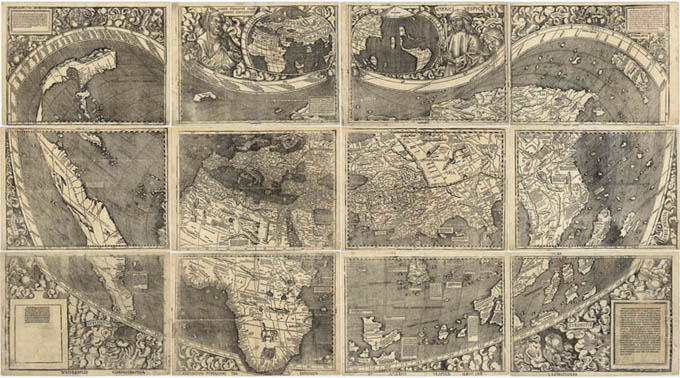
\includegraphics[width=1\textwidth]{graph_and_picture/Waldseemuller_map.jpg}
    \caption{A map}
    \label{chapter1_map_waldseemuller}
\end{figure}


% bibliography
\pagebreak
\bibliographystyle{chicago}
\bibliography{Bibliographies/Paper1.bib}




% If you put main tables/maps/graph, etc. outside the main text but not in Appendix:
\pagebreak
\section*{Tables (if put in the end of the paper)}

\begin{table}[h!]
    \centering
    \begin{tabular}{cccc}
\hline \hline
\multirow{2}{*}{Frequency} &   & \multicolumn{2}{l}{Region}       \\
                           &   & A           & B                  \\
\hline                           
\multirow{2}{*}{Period}    & 1 & 78521          & 3982            \\
                           & 2 & 54246          & 3521            \\
\hline \hline
    \end{tabular}
    \caption{Frequency Table}
    \label{paper1_table_frequency}
\end{table}  




\pagebreak
\begin{subappendices}

\section{The colors on the maps}
\lipsum[10-10]

\section{{The origin of the map}}
\lipsum[11-11]


\end{subappendices}